\documentclass[10pt]{beamer}
\usepackage{color}
\usepackage{graphics}
\usepackage{hyperref}
\usepackage{multimedia}
\usepackage{beamerthemeshadow}
\usepackage{epsfig}
\usepackage{xcolor, colortbl}
\usepackage{array, multirow, multicol}

\definecolor{tun}{rgb}{0.5,0.09,0.17}

\setbeamertemplate{background canvas}[vertical
shading][bottom=blue!10,top=green!20]

\setbeamercovered{dynamic}

\newtheorem{teorema}{Teorema}[section]
\newtheorem{observacion}{Observaci\'on}[section]
\newtheorem{dem}{Demostraci\'on}[section]
\newtheorem{lema}{Lema}[section]
\newtheorem{proposicion}{Proposici\'on}[section]
\newtheorem{hipotesis}{Hip\'otesis}[section]
\newtheorem{definicion}{Definici\'on}[section]
\newtheorem{observation}{observation}[section]
\newtheorem{remark}{remark}[section]
\newtheorem{conclusiones}{\¿Qu\'e se va a avanzar este semestre?}[section]
\newtheorem{final remarks}{final remarks}[section]
\newtheorem{future work collaboration}{future work collaboration}[section]
\usetheme{Darmstadt}
\usecolortheme[named=tun]{structure}
\usefonttheme{professionalfonts}
\usepackage[latin1]{inputenc}
\usefonttheme[onlylarge]{structuresmallcapsserif}
\DeclareMathOperator{\sech}{sech}

\begin{document}

%%%%%%%%%%%%%%%%%%%% PORTADA %%%%%%%%%%%%%%%%%%%%%%%%%%%%

\title{Teor\'ia de perturbaciones para existencia de ciclos l\'imites}

\author {\textcolor[rgb]{0.20,0.50,0.20}{ {Eduardo Ortiz Romero}}}
\institute[Instituto Polit\'ecnico Nacional]{%
Escuela Superior de F\'{i}sica y Matem\'{a}ticas,\\
Instituto Polit\'{e}cnico Nacional.}
\date{Posgrado, Maestr\'ia en Ciencias F\'isico Matem\'aticas}

\colorlet{redshaded}{red!25!bg} \colorlet{shaded}{black!25!bg}
\colorlet{shadedshaded}{black!10!bg}
\colorlet{blackshaded}{black!40!bg}

\colorlet{darkred}{red!80!black}
\colorlet{darkblue}{blue!80!black}
\colorlet{darkgreen}{green!80!black}

\definecolor{lila}{rgb}{0.72,0.00,0.72}

\definecolor{rojo}{rgb}{0.98,0.00,0.00}

\def\radius{1.2cm}
\def\innerradius{0.85cm}

\def\softness{0.4}
\definecolor{softred}{rgb}{1,\softness,\softness}
\definecolor{softgreen}{rgb}{\softness,1,\softness}
\definecolor{softblue}{rgb}{\softness,\softness,1}

\definecolor{softrg}{rgb}{1,1,\softness}
\definecolor{softrb}{rgb}{1,\softness,1}
\definecolor{softgb}{rgb}{\softness,1,1}
\definecolor{lightcopper}{rgb}{0.54, 0.81, 0.94}
\definecolor{brickred}{rgb}{0.8, 0.25, 0.33} 
\definecolor{cadetblue}{rgb}{0.37, 0.62, 0.63}
\definecolor{cadet}{rgb}{0.0, 0.48, 0.65}
\begin{frame}

\includegraphics[scale=0.08]{Img/ipn4.png}
\hfill

\includegraphics[scale=0.3]{Img/esfm4.png}
\titlepage
\end{frame}

%%%%%%%%%%%%%%%%%%%%% ALPHA Y OMEGA LÍMITE %%%%%%%%%%%%%%%%%%%%%%%%%%%%%%

\begin{frame}
    Al conjunto de todos los puntos $\omega$-l\'imite los llamaremos \textbf{Conjunto $\omega$-l\'imite}.\\
    Al conjunto de todos los puntos $\alpha$-l\'imite los llamaremos \textbf{Conjunto $\alpha$-l\'imite}.
\end{frame}

%%%%%%%%%%%%%%%%%%%%%% Teoría de Promediación %%%%%%%%%%%%%%%%%%%%%%%%%%%%%%%

\subsection{Teor\'ia de promediaci\'on}

\begin{frame}
    Se utiliza en sistemas de ecuaciones $2\times 2$ de la forma
    $$X'=\epsilon f(t,X)$$

    El problema se transforma en el sistema 
    $$Y'=\epsilon f_T(t,Y)$$
    donde $f_t$ es el promedio local definido así:
    \begin{definition}
        Sea $f:\mathbb{R}\times\mathbb{R}^p\to\mathbb{R}^n$ continua y $T>0$.
        Definimos:
        $$
            f_T(t,x)=\frac{1}{T}\int_{0}^{T}f(t+\tau,x)d\tau
        $$
        como el promedio local de $f$.
    \end{definition}
\end{frame}

%%%%%%%%%%%%%%%%%%%%%%% Lipschitz %%%%%%%%%%%%%%%%%%%%%%%%%%%%%%%%%%%%%%

\begin{frame}

    Si $\phi:\mathbb{R}\to\mathbb{R}$ es de Lipschitz en $\mathbb{R}$, entonces
	$$
		\abs{\phi(x)-\phi_T(x)}\leq\frac{\lambda T}{2}
	$$
	i.e. $\phi(t)$ es $o(T)$ con respecto a $\phi_T(x)$.
    
\end{frame}

%%%%%%%%%%%%%%%%%%%%%%%   EJEMPLO   %%%%%%%%%%%%%%%%%%%%%%%%%%%%%%%%%

\begin{frame}
    Consideremos la funci\'on $\phi(t)=\sqrt{t^2+1}$, esta funci\'on es de Lipschitz
	con constante $\lambda=1$, calculamos su promedio local con $T=0.5$
    
	\begin{figure}[h]
		\centering
		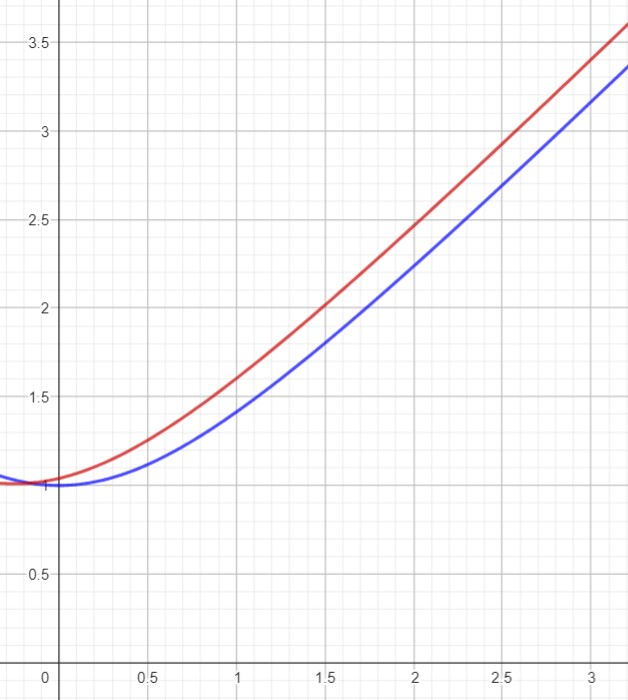
\includegraphics[width=5.5cm]{Img/fl.jpg}
		%\caption{}
	\end{figure}

\end{frame}

\begin{frame}
    La diferencia esta acotada por $M=\frac{\lambda T}{2}=\frac{0.5}{2}=0.25$. 
    En este caso en la 
gr\'afica se puede observar que la diferencia converge a la cota $M$. 
    \begin{figure}[h]
        \centering
        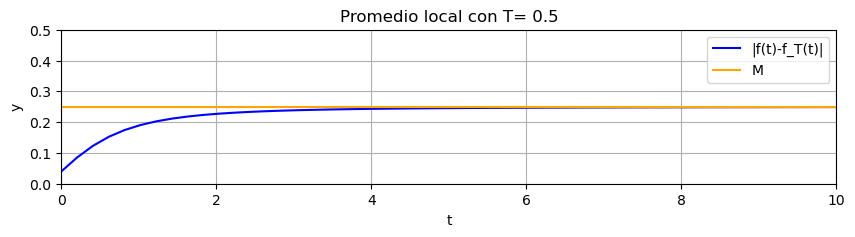
\includegraphics[width=10cm]{Img/d.png}
       % \caption{Diferencia de la Función con la función promediada.}
    \end{figure}
\end{frame}

\begin{frame}
    Es lo mismo pero m\'as barato.
    \begin{figure}[h]
		\centering
		
\includegraphics[width=5cm]{Img/simi.jpg}
		%\caption{}
	\end{figure}
\end{frame}

\begin{frame}
    
    \begin{lemma}
        Consideremos el problema de valor inicial
        $$
            x'=\epsilon f(t,x)
        $$
        $x(0)=x_0$, con $f$ Lipschitz en $x\in D\subseteq\mathbb{R}^n$ y continua
        en $t\in[0,t]$. \\
        Si $y$ es soluci\'on de $y'=\epsilon f_T(t,y)$, $y(0)=x_0$, entonces
        $$
            x(t)-y(t)=o(\epsilon T)
        $$
        p.t. $t=o(\frac{1}{\epsilon})$
    \end{lemma}

    

\end{frame}

%%%%%%%%%%%%%%%%%%% OSCILADOR DE VAN DEL POL %%%%%%%%%%%%%%%%%%%%%%%%%%%%%%%%%%%

\subsection{Oscilador de Van der Pol}
\begin{frame}
\begin{center}
    \textbf{Oscilador de Van der Pol}
\end{center}
La ecuaci\'on del oscilador de Van der Pol describe el comportamiento 
de ciertos sistemas oscilantes no lineales.
Su fundamento f\'isico se basa en el concepto de amortiguamiento no lineal.
$$x''+\epsilon(x^2-1)x'+x=0.$$
Lo transformamos en un sistema de ecuaciones en coordenadas polares
$$
\begin{matrix}
    r'=-\epsilon r \sin^2(\theta)(r^2\cos^2(\theta)-1) \\ 
    \theta' = 1-\epsilon r \sin(\theta)\cos(\theta)(r^2\cos(\theta)-1)
\end{matrix}$$
\end{frame}




%%%%%%%%%%%%%%%%%%%%%%%% PROMEDIACIÓN DEL OSCILADOR DE VAN DER POL %%%%%%%%%%%%%%%%%%%%%%%%

\begin{frame}
    \begin{center}
        \textbf{Promediaci\'on del Oscilador de Van der Pol}
    \end{center}
Definimos
$$\bar{r}'=\bar{f}(\bar{r},\epsilon)=\frac{1}{2\pi}\int_0^{2\pi}r'd\theta$$
Promediamos y el resultado es un sistema m\'as simple.
$$
\begin{matrix}
    \bar{\theta}=2\pi \\
    \\
    \bar{r}=\frac{\epsilon}{8}r(4-r^2)
\end{matrix}
$$

\end{frame}

%%%%%%%%%%%%%%%%%%%%%%%% PLANO FASE %%%%%%%%%%%%%%%%%%%%%%%%%%%%%

\begin{frame}
    \begin{figure}[h]
        \centering
        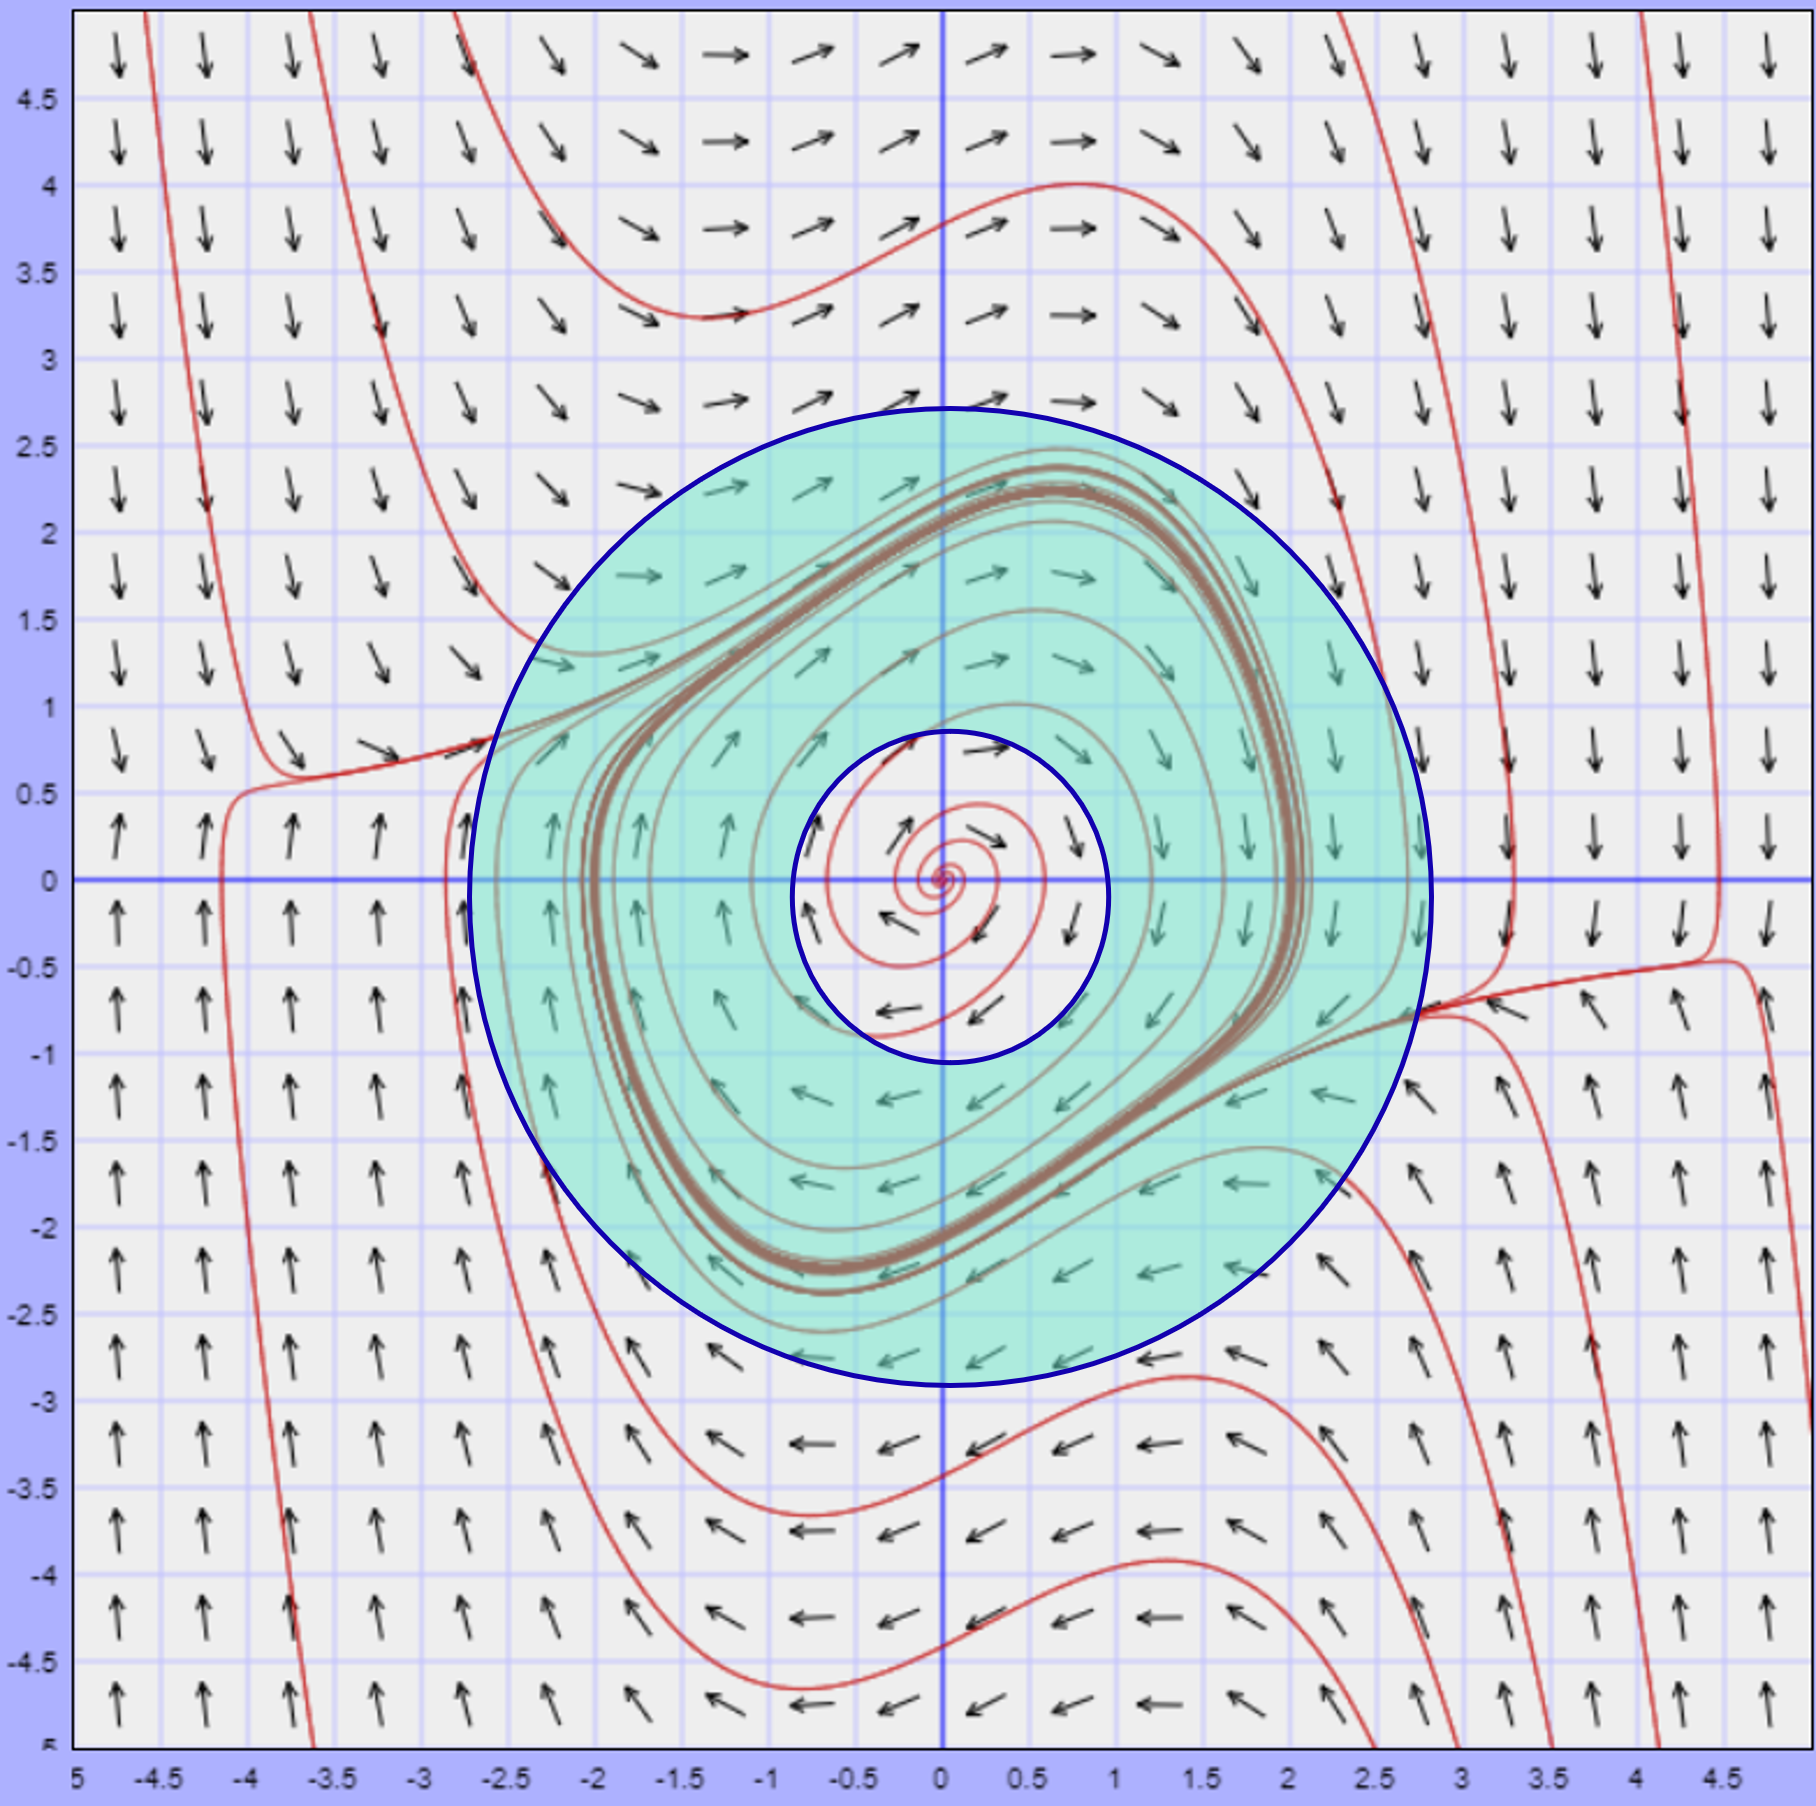
\includegraphics[width=7cm]{Img/vanderpol2.png}
    \end{figure}
\end{frame}

\begin{frame}
    En azul la soluci\'on real, en amarillo el promedio.
    \begin{figure}[h]
		\centering
		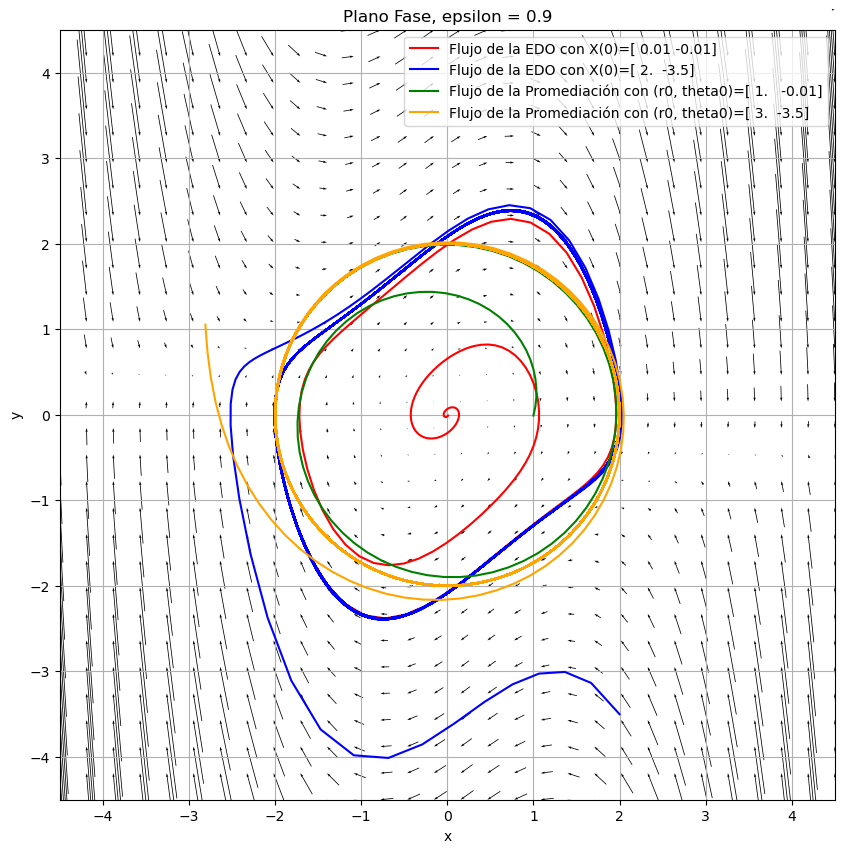
\includegraphics[width=7cm]{Img/ejem.png}
		%\caption{}
	\end{figure}
\end{frame}

\end{document}
